

%We attach unique identifiers to type holes, interpret them as type variables, and infer types for holes with Hindley-Milner \emph{type inference} \cite{MilnerInfer} based on unification \cite{RobinUnification}. The algorithm follows two standard steps, constraint generation and constraint solving by unification.

%The implementation inserts holes automatically, following the \Hazelnut edit action calculus, to guarantee that every editor state has some (possibly incomplete) type.

\section{Introduction}
\label{sec:intro}
\emph{Bidirectional typing} and \emph{type inference} have complementary strengths on type checking and deducing types for programs. \emph{Bidirectional typing} has an understandable resulting system and produces clear error messages at the cost of requiring explicit type annotations \cite{BidirTyping}. \emph{Type inference} allows programmers to omit type annotations, but requires complex constraint solving for type checking and has difficult error messages \cite{typeinferDif}. Besides, programmers are also hard to figure out what type a variable has when it is inferred. This paper develops \emph{type hole inference}, combining benefits of \emph{bidirectional typing} and \emph{type inference}.\par

\citet{HazelnutPOPL} in recent \Hazel work assigns the formal meaning to missing types in incomplete programs as \emph{type holes}, identified as unknown types in gradual type theory \cite{GradualTyping}. Our approach uses bidirectional typing based on the hole system, like \Hazel does, but adds constraint solving as a layer on top to suggest type hole fillings. Take programs in \Hazel environment extended with type hole inference as examples: 
\begin{figure}[htbp]
\centering
  \begin{tabular}[b]{cc}
    \begin{tabular}[b]{c}
      \begin{subfigure}[b]{0.4\columnwidth}
        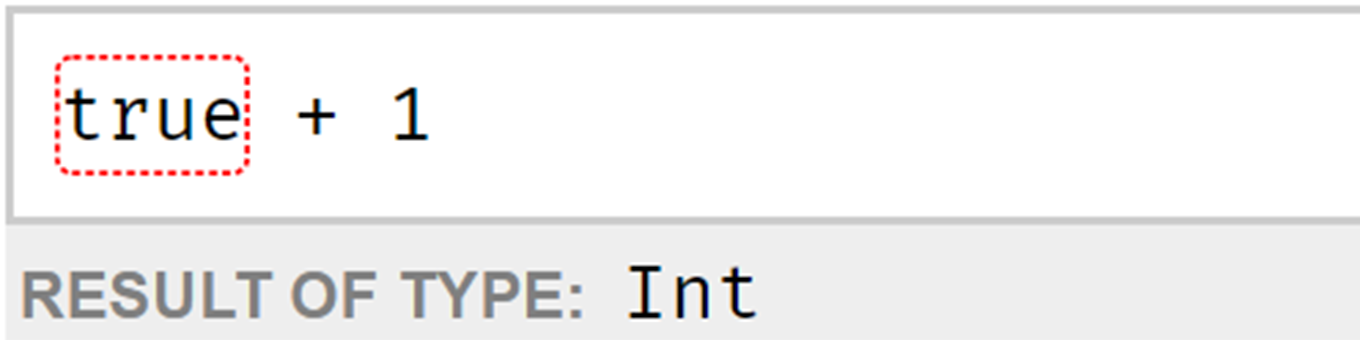
\includegraphics[width=5cm]{3_1.png}
        \caption{Example of static error}
        \label{fig:staticerror}
      \end{subfigure}\\
      \begin{subfigure}[b]{0.4\columnwidth}
        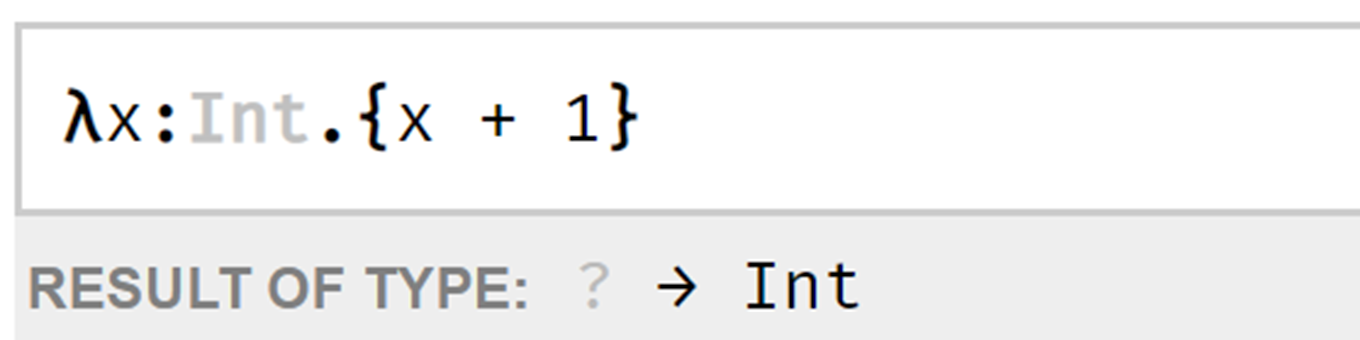
\includegraphics[width=5cm]{4_gray.png}
        \caption{Example of constraint solving success}
		\label{fig:unifsuc}
      \end{subfigure}
    \end{tabular}
    &
     \begin{tabular}[b]{c}
          \begin{subfigure}[b]{0.4\columnwidth}
      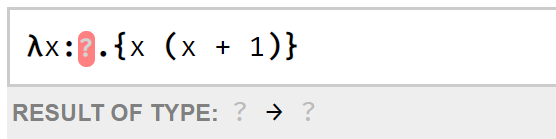
\includegraphics[width=5cm]{unifyfail_2.png}
      \caption{Example of constraint solving failure}
	\label{fig:uniffail}
	\end{subfigure}\\
      \begin{subfigure}[b]{0.4\columnwidth}
        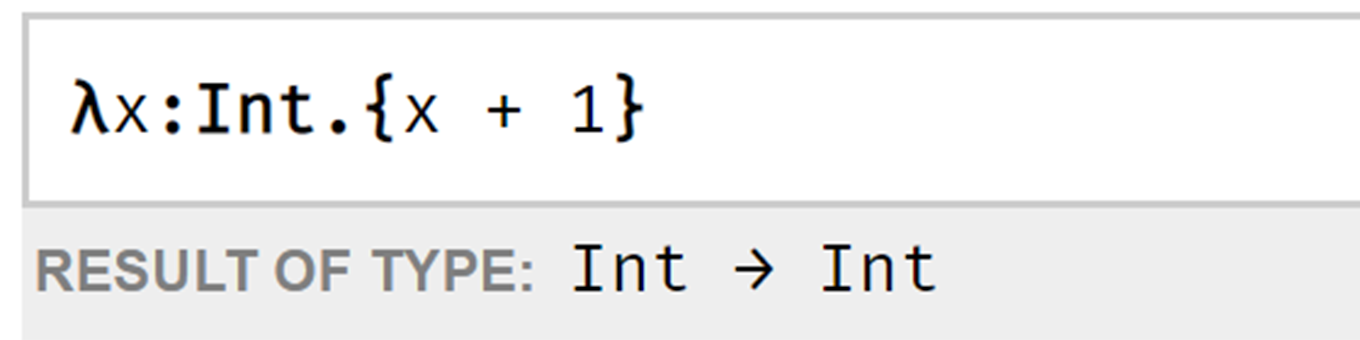
\includegraphics[width=5cm]{4_black.png}
        \caption{Example of filling type holes}
		\label{fig:fillholeeg}
      \end{subfigure}
    \end{tabular}
  \end{tabular}
  \caption{Programs in Hazel environment}
  \vspace{-2px}
\end{figure}
\par Figure ~\ref{fig:staticerror} fails type checking at bidirectional typing, so our system reports a static error. Bidirectional judgements easily trace back the error and indicate the source in the editor with a red box, showing that the operand should be $Int$ type. Bidirectional typing provides clear error message support.\par 
Figure ~\ref{fig:unifsuc} is an example succeeding in both static checking and constraint solving. The bidirectional typing synthesizes the expression to "$\tarr{?}{Int}$" type, with "$?$" standing for hole type. The constraint solver then generates a solution, $[(?,~ Int)]$, for the type hole from the synthesized type. Hence, the type hole is filled with a gray "$Int$" in the editor. The programmer can use a keyboard shortcut to replace the type hole with the suggested type as shown in figure ~\ref{fig:fillholeeg}, and the expression is synthesized to "$\tarr{Int}{Int}$" after replacement. \par

Figure ~\ref{fig:uniffail} is an example failing in constraint solving. Constraints, $(? \sim Int)$ and $(? \sim \tarr{?}{?})$, conflict since the type hole can not be $Int$ and $arrow \, type$ at the same time. In this case, the expression still remains well-typed since $x$ is of hole type. The system postpones type-checking to runtime rather than report a static error.

\emph{Type hole inference} has a simple typing algorithm, simple error messages, and explicit annotations in the same situations that bidirectional typing does. However, programmers don't have to actually fill out those explicit annotations, most of which are type holes inserted and filled by the \emph{type hole inference} automatically as shown in figure ~\ref{fig:unifsuc}. The algorithm treats type holes as unknown types, and regards expressions well-typed until holes are inferred through constraint solving. 
%Besides, types that are generated by constraint solving always relate to a syntactic type hole in the code, so there is always somewhere to display them in the editor.
% The problem is that limited type information for type holes gained through bidirectional typing judgements \cite{HazelLive}. \par

% \citet{HazelnutPOPL} derived \emph{type holes} coinciding with machinery of gradual typing \cite{GraualTyp}, identifying type holes as unknown types. We 

% Inferring types for type holes turns to be a problem of realizing type inference on gradual typing system. 

%  To combine type inference with gradual typing, \citet{GradualInfer} came up an inference algorithm with design space under conditions that three straightforward approaches fail. One simple approach that replaces unknown types with a fresh variable and apply type inference does not work because unexpected static error is triggered when an unknown type is equal to multiple types \cite{GradualInfer}. However, starting from static semantics extended with \emph{holes} gives a new insight to this approach. The type holes corresponding to the unknown type can be filled with hole type to keep programs well-typed when unification fails, and delay type checking for those holes to runtime rather than raise a static error. Our approach is easy to implement by introducing holes into the type inference algorithm \cite{TaplBook}.

% We extended static semantics with \emph{type constraints}, and borrow machinery from unification-based type inference to infer types for type holes by identifying the type hole with the type variable. In particular, our system will not report a static error when unification fails but postpone type-checking for type holes to runtime. This provides an approach to combine \emph{gradual typing} and \emph{type inference}. 
\parahead{Contributions} The contributions of this paper are:
\begin{itemize}
  \item A new bidirectional typing system extended with type constraints. We start from static semantics developed by \citet{HazelnutPOPL}, assigning unique identifiers for type holes and modifying bidirectional judgements for constraint generation in section ~\ref{sec:typinf}.
  \item A new type inference algorithm to handle type holes in section ~\ref{sec:infalg}.
\end{itemize}

%Programmers have to deal with incomplete programs like syntactically malformed edit states during development.